\section{Introduction}

Measurements of anomalies in potential fields, like gravity disturbances and
total-field magnetic anomalies, are widely used in geophysical exploration for
their low cost of acquisition.
These data can be surveyed using ground, airborne, shipborne, or satellite
systems.
During ground surveys, the data are often gathered following irregular paths or
networks along the surface of the terrain, leading to highly variable
elevations in mountainous regions.
Airborne and satellite surveys gather data along flight lines, producing
closely spaced measurements along almost straight lines but with larger spacing
between adjacent lines.
Measurement height can also change because of the vertical movement of the
aircraft.
Processing of the data often involves interpolation onto a regular grid at
constant height, both to improve visualization for interpretation purposes as
well as to prepare the data for further processing and modelling (e.g.,
reduction-to-the-pole, derivative calculations, upward continuation, Euler
deconvolution).

Several methods exist in the literature for interpolation in two dimensions,
for example continuous curvature splines in tension \citep{smith1990},
bi-harmonic (thin-plate) splines \citep{sandwell1987}, and kriging
\citep{hansen1993}.
These general-purpose methods have limitations when it comes to interpolating
potential field data, namely
(i)~they are not able to take into account the variable height of the
observation points and
(ii)~the interpolating functions are not necessarily harmonic, which
is the underlying assumption behind many processing techniques
(e.g., upward continuation and vertical derivatives).

A widely used method for interpolating gravity and magnetic data
is the equivalent sources technique (also known as equivalent layer, radial
basis functions, or Green's functions interpolation).
First introduced by \citet{dampney1969}, the method consists in fitting a model
of finite elementary sources to the data and using this model to predict new
data values.
Besides interpolation, equivalent sources have been used for
reduction-to-the-pole of magnetic data
\citep{silva1986, nakatsuka2006, guspi2009}, upward
continuation \citep{emilia1973, li2010}, joint processing of gravity gradient
data \citep{barnes2011}, modelling the lithospheric magnetic field
\citep{kother2015}, recovering the magnetic induction vector from
total-field magnetic anomalies \citep{li2020}, and more.

It is also worth mentioning the least-squares collocation method
(LSC), which is widely used in geodesy
\citep[][and references therein]{tscherning2015}.
LCS is often applied to combine and interpolate different linear functionals of
the disturbing gravity potential (gravity anomalies, gravity disturbances,
deflections of the vertical, geoid height, et cetera).
Like equivalent sources, collocation also requires the solution of a large
linear system of the order of the number of observed data.
As such, it's practical application suffers from the same computational
challenges.

Many variants of the equivalent sources technique have been proposed, often
attempting to obtain faster or more accurate solutions.
The key factors that vary between them are: (i) the type of source, (ii)
the location of the sources, and (iii) the solution strategy.

The most commonly used type of source is a point mass for gravity or dipole for
magnetics \citep[e.g.,~][]{vonfrese1981, silva1986, mendonca1994,
siqueira2017}.
However, right-rectangular prisms \citep[e.g.,][]{barnes2011, jirigalatu2019,
li2020} and tesseroids \citep{bouman2016} have also been used successfully.
In fact, even point sources with a simple inverse distance function, instead of
actual gravity or magnetic fields, can be used as
equivalent sources \citep{cordell1992}.

The location of sources often follows one of two strategies.
The most common approach is to distribute sources on a regular grid at a
constant depth \citep[e.g.,~][]{leao1989, barnes2011, oliveira2013}.
Alternatively, sources can be placed beneath each data point
\citep[e.g.,~][]{cordell1992, siqueira2017}.
Some recent work by \citet{li2020} places the sources in two overlapping layers
at different depths.

The coefficients of the equivalent source model are often estimated through
damped least-squares.
This imposes a heavy computational load when the number of data points is
large (e.g., airborne and satellite surveys).
To reduce the computational load, \citet{mendonca1994} built the solution
iteratively by incorporating one data point at a time using the ``equivalent
data concept''.
\citet{leao1989} processed the input data using a moving window, only fitting the
data inside the window and predicting observations at its center.
\citet{li2010} and \citet{barnes2011} apply different operations to generate a
sparse representation of the sensitive matrix (respectively, wavelet
compression and quadtree discretization), which significantly improves the
speed of the least-squares solution.
\citet{oliveira2013} parametrized the equivalent layer as a piecewise bivariate
polynomial function, reducing the number of parameters in the solution.
\citet{siqueira2017} developed an iterative solution in which the sensitivity
matrix is transformed into a diagonal matrix with constant terms through the
``excess mass criterion''.
\citet{jirigalatu2019} applied the Gauss-FFT method to speed up the forward
modelling operations and solved the least-squares problem using steepest
descent to avoid calculating the Hessian matrix and solving linear systems.

Many of the existing methods solve under-determined problems, requiring a much
larger number of equivalent sources than the number of data points.
Some achieve greater efficiency by restricting their applications
to specific data types \citep{siqueira2017},
interpolating only on regular grids \citep{leao1989},
or requiring already gridded data \citep{takahashi2020},
to name a few.
Furthermore, many of the optimizations proposed are also complex to implement
in a computer program, limiting their wider adoption.

In the present study,
we propose two strategies for reducing the computational load of
the equivalent sources technique:

\begin{enumerate}
    \item Reduce the number of equivalent sources for oversampled surveys
      through a \emph{block-averaging} strategy while maintaining the quality
      of the solution.
    \item Fit the equivalent source model iteratively along overlapping windows
      using a \emph{gradient boosting} algorithm \citep{friedman2001}.
\end{enumerate}

The first strategy consists in dividing the survey area into horizontal blocks
and assigning a single source to each block, located at the median horizontal
location of the data points.
For airborne, shipborne, and satellite surveys, which are oversampled along
tracks, this can greatly reduce the size of the inverse problem while retaining
the same quality of interpolation.

The gradient boosting algorithm allows us to fit the equivalent source model
iteratively by operating on individual overlapping windows.
As a result, our method solves several much smaller least-squares problems
instead of a large one.
This has some similarities with the strategy used by \citet{leao1989} but
without the requirement for sources and predictions to be on regular grids.

Through tests on synthetic data, we show that:
(i)~the \emph{block-averaged} sources are able to achieve the same accuracy as
other traditional equivalent source layouts while using a fraction of the
number of sources, and
(ii)~the \emph{gradient boosting} algorithm greatly reduces the computational
memory required to fit very large datasets without sacrificing prediction
accuracy.
Finally, a combination of both strategies is used to process a collection of
approximately 1.7 million ground gravity data measurements from Australia.

%%%%%%%%%%%%%%%%%%%%%%%%%%%%%%%%%%%%%%%%%%%%%%%%%%%%%%%%%%%%%%%%%%%%%%%%%%%%%%%

\section{Methodology}

\subsection{The equivalent sources technique}

We will follow the ``generalized equivalent sources'' of \citet{cordell1992}
and assume that any harmonic function $d(\mathbf{p})$ can be approximated by a
sum of $M$ discrete point source effects

\begin{equation}
    d(\mathbf{p})
    =
    \sum\limits_{j=1}^{M} \frac{c_j}{\left\lVert \mathbf{p} - \mathbf{q}_j
    \right\rVert} \ ,
    \label{eq:eql-forward}
\end{equation}

\noindent in which
$\mathbf{p}$ and $\mathbf{q}_j$ are, respectively, the position vectors in a 3D
Cartesian space of data and sources,
$c_j$ is a scalar coefficient related to the point source located at
$\mathbf{q}_j$,
and $\lVert \cdot \rVert$ represents the $\text{L}_2$ norm.
The horizontal and vertical distribution of sources is discussed in
section~\ref{sec:source_distribution}.

In case we have values of the harmonic function at $N$ discrete points
$\{\mathbf{p}_1\ \mathbf{p}_2\ \ldots\ \mathbf{p}_N\}$,
we can write a set of $N$ equations of the form

\begin{equation}
    d_i
    =
    \sum\limits_{j=1}^{M} \frac{c_j}{\left\lVert \mathbf{p}_i - \mathbf{q}_j
    \right\rVert}
    \quad \forall i=1,2,\ldots,N
    \ ,
    \label{eq:forward-sum}
\end{equation}

\noindent where $d_i$ is the calculated value at point $\mathbf{p}_i$.
These equations can also be expressed in matrix form as

\begin{equation}
    \mathbf{d} = \mathbf{A} \mathbf{c} \ ,
    \label{eq:linear-problem}
\end{equation}

\noindent where $\mathbf{d}$ is a column vector containing the $N$ predicted
values at the observation points,
$\mathbf{c}$ is a column vector containing the $M$ coefficients $c_j$,
and $\mathbf{A}$ is the $N \times M$ Jacobian matrix,
whose elements are

\begin{equation}
    a_{ij} = \frac{1}{\left\lVert\mathbf{p}_i - \mathbf{q}_j\right\rVert}
\end{equation}

For a given set of $N$ observed data $\mathbf{d}^o$,
we can find a least-squares solution to
Eq.~\ref{eq:linear-problem} and obtain the values of
$\mathbf{c}$ that best fit the observations.
These coefficients can, in turn, be used to predict the value of the harmonic
function at any other point outside of the sources by evaluating
Eq.~\ref{eq:eql-forward}.
Gridding and upward continuation can thus be achieved by predicting values on
points that fall on a regular grid or at different heights, respectively.


\subsection{Damped least-squares solution}
\label{sec:eql_inversion}

We can obtain the values of the source coefficients $\mathbf{c}$ that best
fit the observed field values $\mathbf{d}^o$ by minimizing the goal function

\begin{equation}
    \phi(\mathbf{c}) =
    \left[\mathbf{d}^o - \mathbf{A}\mathbf{c}\right]\trans
    \mathbf{W}
    \left[\mathbf{d}^o - \mathbf{A}\mathbf{c}\right]
    + \lambda_d\ \mathbf{c}\trans\mathbf{c}
    \ ,
    \label{eq:misfit-unscaled}
\end{equation}

\noindent where
$\mathbf{W}$ is a $N \times N$ diagonal matrix of data weights and
$\lambda_d$ is a positive \emph{damping} parameter with the same units as the
Jacobian matrix elements.
The second term on the right-hand side of Eq.~\ref{eq:misfit-unscaled} is the
zeroth-order Tikhonov regularization \citep{tikhonov1977}, also known as a
damping regularization, that is used to stabilize the solution.

The damping parameter controls the amount of regularization that will be
applied.
An overly large value would generate a smooth solution that fails to reproduce
the high frequency components of the data, while an overly small value would
result in over-fitting, thus failing to produce realistic interpolation results
\citep{martinez2016}.
The range of acceptable values for the damping parameter $\lambda_d$ will
depend on the values of the Jacobian matrix $\mathbf{A}$ and the coefficients.
Consequently, this range will vary (often dramatically) between datasets,
making it difficult to choose an appropriate value in practice.

To solve this issue, we first scale the Jacobian matrix so that its elements
are dimensionless and each column has unit variance.
We define a diagonal matrix $\mathbf{S}$

\begin{equation}
    \mathbf{S} =
    \begin{bmatrix}
      \sigma_1 & 0 & \cdots &0 \\
      0 & \sigma_2 & \cdots &0 \\
      \vdots & \vdots & \ddots & \vdots \\
      0  & 0 & \cdots & \sigma_M
    \end{bmatrix}_{M \times M}
    ,
\end{equation}

\noindent in which $\sigma_j$ is the standard deviation of the $j$-th column of
$\mathbf{A}$.
We then write the forward problem in Eq.~\ref{eq:linear-problem} as

\begin{equation}
    \mathbf{d}
    =
    \mathbf{A} \mathbf{S}\inv \mathbf{S} \mathbf{c}
    =
    \left[
        \mathbf{A} \mathbf{S}\inv
    \right]
    \left[
        \mathbf{S} \mathbf{c}
    \right]
    =
    \mathbf{B} \mathbf{m}
\end{equation}

\noindent where $\mathbf{B} = \mathbf{A} \mathbf{S}\inv$ is the scaled and
dimensionless Jacobian matrix
and $\mathbf{m} = \mathbf{S} \mathbf{c}$ is a vector containing scaled
coefficients with the same units as the data.

The goal function defined in Eq.~\ref{eq:misfit-unscaled} can be
rewritten as

\begin{equation}
    \phi(\mathbf{m}) =
    \left[\mathbf{d}^o - \mathbf{B}\mathbf{m}\right]\trans
    \mathbf{W}
    \left[\mathbf{d}^o - \mathbf{B}\mathbf{m}\right]
    + \lambda\ \mathbf{m}\trans\mathbf{m}
    \ ,
    \label{eq:misfit}
\end{equation}

\noindent where $\lambda$ is a \emph{dimensionless} damping parameter and
regularization is applied on the scaled coefficients $\mathbf{m}$ instead of
$\mathbf{c}$.
Using a dimensionless damping parameter allows us to narrow the range of values
of $\lambda$ that would generate the most accurate predictions, irrespective
of the dataset and its units.
From experience, we recommend searching for suitable $\lambda$ values between
$10^{-6}$ and $10^{4}$ varying by order-of-magnitude.
The choice of the damping and other hyper-parameters, like the source depth,
could be done through well-established statistical methods, such as
cross-validation.

The vector of scaled coefficients $\hat{\mathbf{m}}$ that minimizes the goal
function can be found by solving the \emph{normal equation system}
\citep{menke1989}

\begin{equation}
    \left[
      \mathbf{B}\trans \mathbf{W} \mathbf{B} + \lambda \mathbf{I}
    \right]
    \hat{\mathbf{m}} =
    \mathbf{B}\trans\mathbf{W}
    \mathbf{d}^o.
    \label{eq:least_squares_solution}
\end{equation}

Once the scaled coefficients are obtained, the estimated unscaled coefficients
$\hat{\mathbf{c}}$ can be calculated by removing the scaling factor

\begin{equation}
    \hat{\mathbf{c}} = \mathbf{S}\inv \hat{\mathbf{m}} \ .
\end{equation}

\noindent The forward modeling operations used to perform predictions
(e.g., for interpolation and upward continuation) are left unchanged by
using vector $\hat{\mathbf{c}}$ instead of $\hat{\mathbf{m}}$.


\subsection{Gradient boosting}

Gradient boosting was first introduced by \citet{friedman2001, friedman2002} as
a method for fitting additive parametric models of the form

\begin{equation}
    d = \sum_{k=1}^K \alpha_k f(\mathbf{c}_k),
\end{equation}

\noindent where $\alpha_k$ is a scalar coefficient called the \emph{step-size}
and $f$ is a function of the parameter vector $\mathbf{c}_k$.
For linear problems, these additive models can be written as the matrix
equation

\begin{equation}
    \mathbf{d} = \sum_{k=1}^K \mathbf{A}_k \mathbf{c}_k \ .
    \label{eq:gb-linear-model}
\end{equation}

\noindent Because of the linearity of the $f(\mathbf{c}_k)$ functions, the
$\alpha_k$ step-size parameters can be incorporated into the parameter vector
$\mathbf{c}_k$.

We can transform our equivalent source problem in
Eq.~\ref{eq:linear-problem} into an additive model by following these
steps:

\begin{enumerate}
  \item Define a set of $M$ equivalent sources distributed throughout the
    survey area (see section \ref{sec:source_distribution} for details).
  \item Define a set of $K$ overlapping windows of equal size that cover the
    survey area.
  \item Create $K$ separate sets of equivalent sources, one for each window.
    Each set will be formed by the portion of the original $M$ sources that
    fall inside the respective window.
    Since the windows overlap, the total number of sources from all sets will
    be greater than $M$.
  \item Define vector $\mathbf{c}_k$ as the $M_k$ coefficients of the
    equivalent sources of the $k$-th window.
  \item Define matrix $\mathbf{A}_k$ as the $N \times M_k$ Jacobian matrix
    between the sources in the $k$-th window and all $N$ data points of the
    survey.
  \item Model the predicted data as a superposition of the effects of the $K$
    separate sets of equivalent sources (i.e., Eq.~\ref{eq:gb-linear-model}).
\end{enumerate}

The gradient boosting algorithm works by fitting each component of the
additive model, one at a time, to the residuals of the previous component.
\citet{friedman2001} demonstrates that this corresponds to a steepest-descent
optimization in the so-called ``function space''.
The adaptation of the gradient boosting method to find the damped least-squares
solutions for the $K$ parameter vectors $\mathbf{c}_k$ in
Eq.~\ref{eq:gb-linear-model} is presented in
Algorithm~\ref{alg:gradient_boosting}.

\begin{algorithm}[!h]
  \DontPrintSemicolon
  \setstretch{1.5}
  Define the residual vector $\mathbf{r}_{0} = \mathbf{d}^o$ \;
  \For{ $k = 1$ \KwTo $K$ }{


    Calculate the $N \times M_k$ Jacobian matrix $\mathbf{A}_k$
    \;

    $\mathbf{B}_k = \mathbf{A}_k \mathbf{S}_k\inv$
    \nllabel{alg:scale}
    \;

    $
     \hat{\mathbf{m}}_k = \left[\mathbf{B}_k\trans \mathbf{W}_k \mathbf{B}_k +
     \lambda \mathbf{I} \right]\inv \mathbf{B}_k\trans \mathbf{W}_k
     \mathbf{r}_{k-1}
    $
    \nllabel{alg:fit}
    \;

    $\hat{\mathbf{c}}_k = \mathbf{S}_k\inv \hat{\mathbf{m}}_k$
    \nllabel{alg:unscale}
    \;

    $\mathbf{d}_k = \mathbf{A}_k \hat{\mathbf{c}}_k$
    \nllabel{alg:predicted}
    \;

    $\mathbf{r}_k = \mathbf{r}_{k - 1} - \mathbf{d}_k$
    \nllabel{alg:residual}
    \;
  }
  \BlankLine
  \setstretch{1}
  \caption{Gradient boosting solution for damped least-squares regression.}
  \label{alg:gradient_boosting}
\end{algorithm}

After all $\mathbf{c}_k$ coefficients vectors are estimated, we can predict the
effect of the additive equivalent source model on any point through the
summation

\begin{equation}
    d(\mathbf{p}) =
    \sum\limits_{k=1}^K \sum\limits_{j=1}^{M_k}
    \frac{{c_k}_j}{\left\lVert \mathbf{p} - {\mathbf{q}_k}_j \right\rVert}
    \ ,
    \label{eq:eql-forward-gb}
\end{equation}

\noindent
in which ${c_k}_j$ is the $j$-th element of the $\mathbf{c}_k$ vector and the
${\mathbf{q}_k}_j$ is the position vector of the $j$-th source of the $k$-th
window.

To improve the convergence of the algorithm, \citet{friedman2002} suggests
introducing randomness into the fitting process. We achieve this by randomizing
the order in which the $K$ windows are used in the gradient boosting algorithm.
Section~\ref{sec:gb_interpolation} explores the effect of randomization in the
convergence rate of the algorithm and the accuracy of the interpolation.

The $\mathbf{A}_k$ matrices have only $N \times M_k$ elements
(where $M_k$ is the number sources on the $k-$th window), which can be
considerably smaller than the $N \times M$ elements of $\mathbf{A}$.
Therefore, the gradient boosting method allows us to fit
equivalent source models that would produce Jacobian matrices that are larger
than the available computer memory.
Furthermore, we can increase or decrease the size of the overlapping windows as
needed depending on the number of sources in the model and the available
computer memory.

We can improve the efficiency of the algorithm further by:

\begin{enumerate}
  \item Using only the $N_k$ data points that fall within the $k$-th window for
    fitting the sources (steps \ref{alg:scale} and \ref{alg:fit} of
    algorithm~\ref{alg:gradient_boosting}).
    By doing so, we can replace the $N \times M_k$ Jacobian matrix $\mathbf{A}_k$
    with the smaller $N_k \times M_k$ matrix $\tilde{\mathbf{A}}_k$.
    We still use all $N$ data points when calculating the predicted data and
    residuals (steps \ref{alg:predicted} and \ref{alg:residual} of
    algorithm~\ref{alg:gradient_boosting}).
  \item The forward modeling operation performed in step \ref{alg:predicted}
    can be done by a summation (Eq.~\ref{eq:forward-sum}) instead of a
    matrix-vector product, which allows us to avoid computing and storing the
    larger $N \times M_k$ matrix $\mathbf{A}_k$ at any point.
\end{enumerate}

Algorithm~\ref{alg:gradient_boosting_window} is the final
\textit{gradient-boosted equivalent sources algorithm} which incorporates these
changes.
Figure~\ref{fig:gradient-boosting-schematics} shows a sketch of the algorithm
steps applied a set of observation points that simulate a ground survey and
locating one source below each data point.

\begin{algorithm}[!h]
  \DontPrintSemicolon
  \setstretch{1.5}
  Define the residual vector $\mathbf{r}_{0} = \mathbf{d}^o$ \;
  \For{ $k = 1$ \KwTo $K$ }{

    Select weights $\tilde{\mathbf{W}}_k$ and residuals
    $\tilde{\mathbf{r}}_{k - 1}$ for data points inside the $k$-th window
    \;

    Calculate Jacobian matrix $\tilde{\mathbf{A}}_k$ with data points and
    sources inside the $k$-th window
    \;

    $\mathbf{B}_k = \tilde{\mathbf{A}}_k \mathbf{S}_k\inv$
    \;

    $
     \hat{\mathbf{m}}_k = \left[
     \mathbf{B}_k\trans \tilde{\mathbf{W}}_k \mathbf{B}_k +
     \lambda \mathbf{I} \right]\inv \mathbf{B}_k\trans \tilde{\mathbf{W}}_k
     \tilde{\mathbf{r}}_{k-1}
    $
    \;

    $\hat{\mathbf{c}}_k = \mathbf{S}_k\inv \hat{\mathbf{m}}_k$
    \;

    Calculate $ \mathbf{d}_k $, where
    $
    {d_k}_i
    =
    \sum\limits_{j=1}^{M_k} \dfrac{{c_k}_j}{\left\lVert \mathbf{p}_i -
        {\mathbf{q}_k}_j
    \right\rVert}
    \quad \forall\ i=1\ \text{to}\ N
    $
    \;

    $\mathbf{r}_k = \mathbf{r}_{k - 1} - \mathbf{d}_k$
    \;
  }
  \BlankLine
  \setstretch{1}
  \caption{Gradient-boosted equivalent sources algorithm.}
  \label{alg:gradient_boosting_window}
\end{algorithm}

\begin{figure*}[tb]
    \centering
    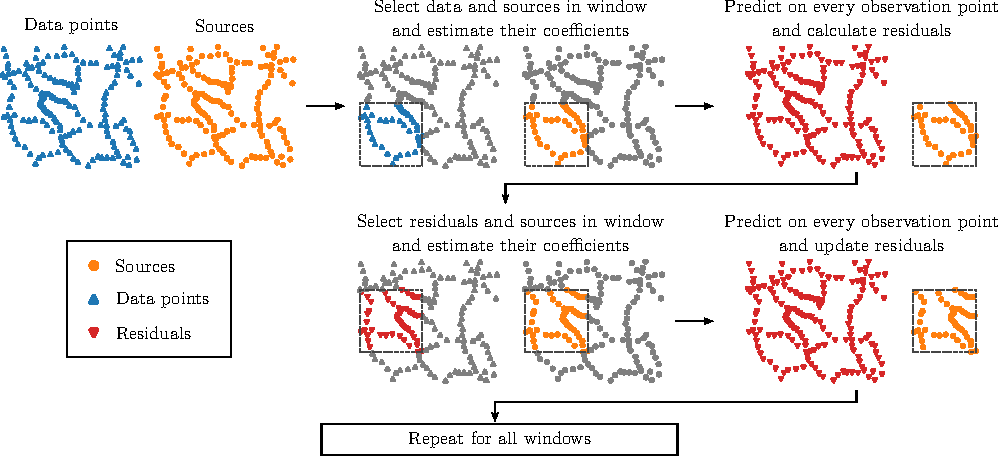
\includegraphics[width=\linewidth]{figs/gradient-boosting-schematics.pdf}
    \caption{
        Sketch of the gradient-boosted equivalent source algorithm.
        Data points are represented by blue upwards-facing triangles,
        equivalent sources by orange dots, data residuals by red downwards-facing
        triangles, and the current window by black dashed lines.
        The algorithm starts by selecting the data and sources
        inside the first window and estimating the source coefficients
        using the selected data points.
        Then, the effect of the estimated sources is predicted on all data
        points and used to calculate the residuals.
        Another window is used to select residuals and sources and
        estimate the coefficients using the selected residuals instead of the
        original data.
        Again, the effect of the estimated sources is predicted on all data points
        and the residuals are updated.
        These steps are repeated for every window in a randomized order.
    }
    \label{fig:gradient-boosting-schematics}
\end{figure*}

It is worth noting that two sets of equivalent sources obtained through two
adjacent overlapping windows have some portion of the sources on the same
locations, specifically the ones that fall on the intersection between the two
windows.
We can interpret this as the gradient-boosting algorithm fitting the source
coefficients multiple times: one time for every window that covers each source.
This fact can be exploited in order to save computer memory.
Instead of storing all of the $\mathbf{c}_k$ vectors
(Eq.~\ref{eq:gb-linear-model}), we can initialize a single $\mathbf{c}$ vector
with zeros, where each element represents the coefficient of each one of the
original $M$ sources.
After each iteration of the gradient-boosting algorithm, we add the estimated
coefficients $\hat{\mathbf{c}}_k$ to the corresponding elements of vector
$\mathbf{c}$.
Because the forward modelling function is linear, we can safely compute the
resulting field through Eq.~\ref{eq:eql-forward} instead of
Eq.~\ref{eq:eql-forward-gb}.
This way, the memory needed to store the entire set of estimated coefficients
is limited to a single vector of $M$ elements.

Our gradient boosting algorithm for overlapping windows is similar to the
``bootstrap inversion'' used in \citet{vonfrese1988}, which also iteratively
fits portions of an equivalent source model to the data residuals.
The key differences are that in our method:
(i)~the sources in the overlapping portions of the windows are fitted more than
once, allowing the algorithm to self-correct for poor solutions to any given
window;
(ii)~we use only data points within the window when fitting, what enables the
use of larger datasets.



\subsection{Location of sources}
\label{sec:source_distribution}

The ideal number of sources and their locations, both horizontally and
vertically, has been debated since the inception of the equivalent sources
technique with \citet{dampney1969}.
The choices made regarding these parameters can play an important role on the
accuracy of the predictions and the computational resources needed to estimate
the source coefficients.
An ideal distribution of sources should simultaneously be able to reproduce the
measured data on the survey points, make accurate predictions on non-surveyed
locations, and minimize the required computational resources.

A large number of evenly distributed sources along the survey region are
capable of reproducing the observed data.
Nevertheless, the computational load can be prohibitive and such
underdetermined problems are prone to overfitting the data, leading to poor
predictive power when interpolating and extrapolating.
On the other hand, using few sources will reduce the computational requirements
but the model may be incapable of reproducing the full spectral content of the
measured data.

Particular survey characteristics also play a role in the choice of equivalent
source distribution.
In a ground survey, observations are usually located along irregular paths and
scattered points.
The coverage of the survey region is often uneven, leaving large areas without
any observation.
On the other hand, observations from airborne surveys are located along almost
straight and closely spaced flight lines.
Measurements are usually taken at a high temporal frequency, leading to
observation points along the flight lines that are several times closer to each
other than the flight line spacing.
This creates a bias in the sampling, which can cause aliasing artifacts in
gridded products.

\subsubsection{Horizontal source layouts}

\begin{figure*}[tb]
    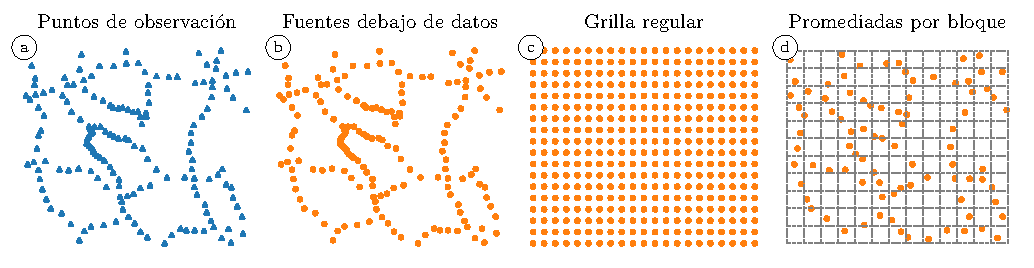
\includegraphics[width=\linewidth]{figs/source-layouts-schematics.pdf}
    \caption{
        Sketch of different horizontal layouts for equivalent source models.
        Blue points represent the locations of observations and orange points
        represent the locations of equivalent sources according to different
        layout strategies.
        (a)~Set of \SourceLayoutsSchematicsObservations{} observation points
        that simulate a ground survey.
        (b)~Location of the \SourceLayoutsSchematicsSourceBelowData{} sources
        obtained through the \emph{sources below data} layout.
        (c)~Location of the \SourceLayoutsSchematicsGridSources{} sources
        obtained through the \emph{regular grid} layout.
        (d)~Location of the \SourceLayoutsSchematicsBlockAveragedSources{}
        sources obtained through the \emph{block-averaged sources} layout.
        Grey dashed lines represent the spatial blocks within which the median
        observation location is calculated.
    }
    \label{fig:source_layouts}
\end{figure*}

The most widely used layouts for distributing equivalent sources horizontally
are:

\begin{enumerate}
  \item
    \emph{Sources below data points}: one equivalent source is placed at the
    horizontal location of each data point (Fig.~\ref{fig:source_layouts}b).
    Therefore, the number of sources is equal to the number of observations
    ($M=N$).
  \item
    \emph{Regular grid}: a homogeneous distribution of point sources below the
    survey region (Fig.~\ref{fig:source_layouts}c). A padding region is often
    added to help reduce edge effects. In practice, it often leads to
    underdetermined problems since a large number of sources is required
    ($M>N$).
\end{enumerate}

For ground surveys, the \emph{regular grid} layout needs a sufficiently
small grid spacing to be able to fit the observed data.
This creates an unnecessarily large number of sources in areas where no
observations exist.
In contrast, the \emph{sources below data} layout is more likely to accurately
fit the observed data with many fewer sources, reducing the computational load.
But when applied to airborne surveys, the \emph{sources below data} layout may
place an undesirably large number of sources along the flight paths.
This could lead to aliasing effects on the predicted values, such as the
stripes parallel to flight lines that are often observed when gridding airborne
magnetic data.
The \emph{regular grid} layout can avoid this effect by evenly
distributing sources and using a continuous source layer (e.g.,
right-rectangular prisms or tesseroids).

We propose a new way of distributing equivalent sources horizontally that could
simultaneously reduce the computational load and mitigate some of the drawbacks
of existing layouts.
In the \emph{block-averaged sources} layout,
point sources are placed in the average
position of data points that fall within specified spatial blocks
(Fig.~\ref{fig:source_layouts}d).
This is done by:

\begin{enumerate}
    \item Dividing the survey region into rectangular blocks of equal size.
    \item \label{item:median-position} Computing the median horizontal position
        of the observation points that fall inside each block. Blocks without
        any observation point are omitted.
    \item Assign one point source to each of the median horizontal positions
      calculated in step \ref{item:median-position}.
\end{enumerate}

The number of sources created by this new layout will be less than the number
of observations if the block size is chosen appropriately (i.e., making sure
that blocks are large enough to contain more than a single data point).
The overdetermined problem that arises from this layout has a lower
computational load and is less prone to overfitting the data since the model
complexity is lower.
Moreover, the block averaging process can balance the spacing between sources
along a flight line and between adjacent lines, helping to reduce aliasing
effects in the generated grids.
In Section~\ref{sec:synthetic_distributions}, we demonstrate through tests on
synthetic data that the block-averaged sources layout is able to interpolate
with comparable accuracy to other layouts while using a fraction of the
equivalent sources.


\subsubsection{Depth of sources}

\begin{figure*}[tb]
    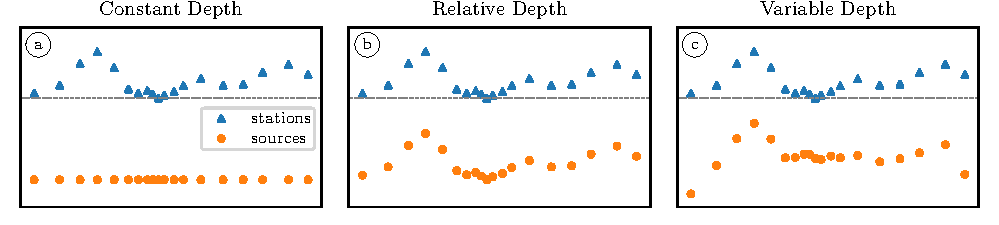
\includegraphics[width=\linewidth]{figs/depth_types.pdf}
    \caption{
        Examples of different strategies for assigning depths to equivalent
        sources.
        Here we assign one source for each
        observation point, located at the same horizontal coordinates as the
        data points.
        Source depths are
        (a)~a \emph{constant depth} at a chosen vertical coordinate,
        (b)~a \emph{relative depth} determined by uniformly shifting downward
        the vertical coordinate of data points,
        and
        (c)~a \emph{variable depth} determined by shifting the vertical
        coordinates of the observation points by an amount proportional to the
        average distance to neighbouring sources.
        The distance between data points and their respective sources (a)
        depends on observation height, (b) is constant, and (c) is proportional
        to the horizontal distribution of sources.
        Notice how the closely spaced sources in the middle of the profile (c)
        are shallower than their counterparts in (b).
    }
    \label{fig:depth_types}
\end{figure*}

It is widely known from potential theory that the depth of a point source
influences the wavelength of the observed field at the surface.
This makes the source depth a key parameter affecting the outcome of
interpolation and other operations done with equivalent sources.
Several different strategies for assigning the depths of equivalent sources
have been proposed in the literature.
Here, we will highlight the following (Fig.~\ref{fig:depth_types}):

\begin{enumerate}
  \item
    \emph{Constant depth}:
    The simplest option is to locate all sources at the same depth
    (Fig.~\ref{fig:depth_types}a).
    If the measurements were taken at significantly different altitudes, some
    measurements will be more distant to the sources than others,
    which may create problems for reproducing short wavelengths in high
    altitude points.
 \item
    \emph{Relative depth}:
    The depths of sources are determined by shifting the vertical coordinate of
    data points downward by a fixed amount (Fig.~\ref{fig:depth_types}b).
    The sources will not all be at the same vertical coordinate, but they will
    all be at the same vertical distance from the observation points.
 \item
    \emph{Variable depth}:
    The depths of sources are proportional to the horizontal distance to the
    nearest neighbouring data points or sources (Fig.~\ref{fig:depth_types}c).
    Different variations of this strategy have been proposed before, for
    example \citet{cordell1992}, \citet{guspi2004}, and \citet{guspi2009}.
    The rationale for this strategy is that if a survey has data points
    clustered in some areas, we may
    want the sources below those areas to be shallower in order to preserve the
    shorter wavelengths that can be measured.
\end{enumerate}

Our approach to the \emph{variable depth} strategy will be:

\begin{equation}
  z = z_{obs} + \Delta z + \alpha h,
  \label{eq:variable_depth}
\end{equation}

\noindent
in which $z$ is the vertical coordinate (positive downwards) of an equivalent
source,
$\Delta z$ is a relative depth shift that is the same for all sources,
$\alpha$ is an dimensionless depth factor,
$h$ is the median horizontal distance to the $k$ nearest neighbouring sources,
and
$z_{obs}$ is a vertical observation coordinate that will depend on the
horizontal layout strategy.
For \emph{sources below data}, it is the vertical coordinate of the data point
corresponding to the given source.
For \emph{regular grid}, it can be interpolated from the vertical coordinates
of all data points.
Finally, for \emph{block-averaged sources} it will be the median vertical
coordinate of the data within the corresponding block.

In Section~\ref{sec:synthetic_distributions}, we test the effectiveness each of
these strategies on synthetic data.

%%%%%%%%%%%%%%%%%%%%%%%%%%%%%%%%%%%%%%%%%%%%%%%%%%%%%%%%%%%%%%%%%%%%%%%%%%%%%%%

\section{Tests on synthetic data}

\begin{figure*}[tb]
    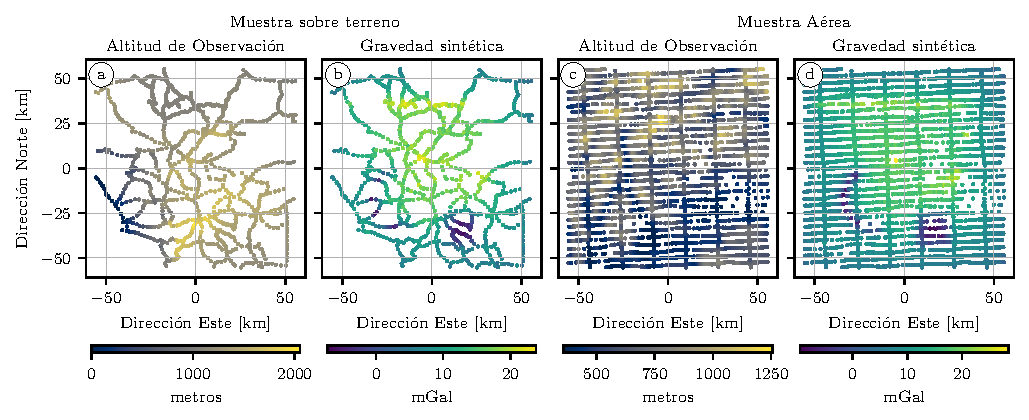
\includegraphics[width=\linewidth]{figs/synthetic-survey-layouts.pdf}
    \caption{
        Observation heights and gravity values for the synthetic ground (a-b)
        and airborne (c-d) surveys.
        Heights are given in meters above the zero height plane.
        The synthetic gravity data are contaminated with pseudo-random Gaussian
        noise with zero mean and \SurveyNoise{} standard deviation.
    }
    \label{fig:synthetic-layouts}
\end{figure*}

\begin{figure}[tb]
    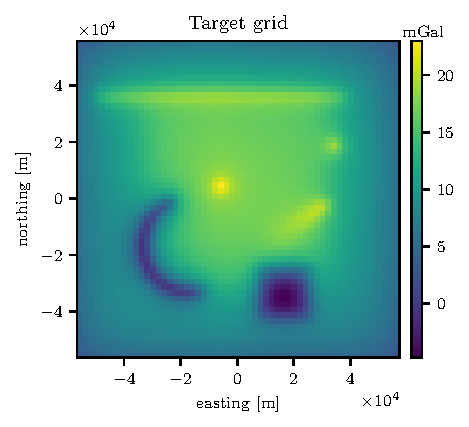
\includegraphics[width=\linewidth]{figs/target-grid.pdf}
    \caption{
        Pseudo-color map of the target grid of synthetic gravity data. The grid
        is composed of \TargetEastingSize{}$\times$\TargetNorthingSize{} points
        with a spacing of \TargetSpacing{}. The grid height is \TargetHeight{}
        above the zero height plane.
    }
    \label{fig:synthetic-target}
\end{figure}

We have used synthetic gravity datasets to test the interpolation accuracy of
the difference horizontal and vertical source distribution strategies as well
as the gradient-boosted equivalent sources method.
To generate the data, we created a model of \NPrisms{} right-rectangular
prisms,
distributed in a \ModelEasting{}$\times$\ModelNorthing{} area with depths
varying between \ModelDepth{} and zero.
The density contrast of prisms ranges from \ModelMinDensity{} to
\ModelMaxDensity{}.
The model includes prisms of different shapes, sizes, and depths to create
gravity disturbances with a variety of wavelengths.

We created two synthetic datasets from the model, one simulating a ground
survey and another an airborne acquisition (Fig.~\ref{fig:synthetic-layouts}).
To create the synthetic ground survey, we selected measurement positions from a
portion of a public domain gravity dataset for Southern Africa, available
through the NOAA National Centers for Environmental Information (NCEI).
For the synthetic airborne survey, we used a portion of the Great Britain
Aeromagnetic Survey acquired by Hunting Geology and Geophysics Ltd and Canadian
Aeroservices Ltd between 1955 and 1965 and made publicly available by the
British Geological Survey (BGS).
In both cases, we rescaled the horizontal coordinates of each survey portion to
span an area of \SurveyEasting{}$\times$\SurveyNorthing{}, matching the model
dimensions.
The ground survey contains \GroundSurveyPoints{} observations distributed at
heights between \GroundSurveyMinHeight{} and \GroundSurveyMaxHeight{}
(Fig.~\ref{fig:synthetic-layouts}a).
The airborne survey has \AirborneSurveyPoints{} observations at heights between
\AirborneSurveyMinHeight{} and \AirborneSurveyMaxHeight{}
(Fig.~\ref{fig:synthetic-layouts}c).

The vertical component of the gravitational acceleration generated by the
model was computed  using the method of \citet{nagy2000, nagy2002}
with recent modifications by \citet{fukushima2020},
as implemented in the open-source software Harmonica \citep{harmonica2020}.
We generated a \emph{target grid} of
\TargetEastingSize{}$\times$\TargetNorthingSize{} points with a spacing of
\TargetSpacing{} and located \TargetHeight{} above the zero height plane
(Fig.~\ref{fig:synthetic-target}) to serve as a reference when calculating the
interpolation error.
We then generated synthetic ground (Fig.~\ref{fig:synthetic-layouts}b) and
airborne (Fig.~\ref{fig:synthetic-layouts}d) data to which we added
pseudo-random Gaussian noise with zero mean and \SurveyNoise{} standard
deviation.


\subsection{Source distribution strategies}
\label{sec:synthetic_distributions}

\begin{figure*}[p]
    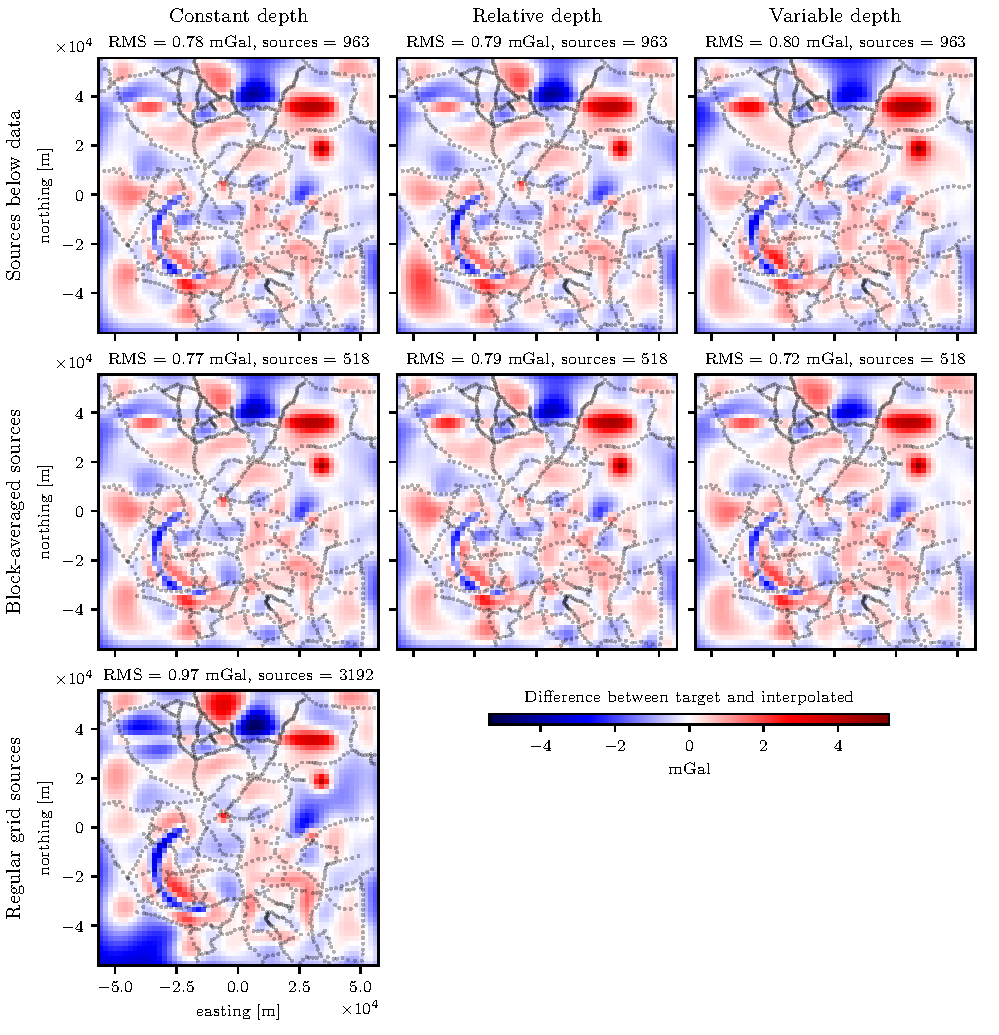
\includegraphics[width=\linewidth]{figs/ground_survey_differences.pdf}
    \caption{
        Pseudo-color maps of the differences between the target grid and the
        interpolated synthetic ground survey data produced by each source
        distribution strategy.
        The black dots represent the horizontal location of the synthetic data
        points. The RMS error and total number of equivalent sources is
        reported for each strategy at the top of the respective maps.
    }
    \label{fig:ground-survey-differences}
\end{figure*}

\begin{figure*}[p]
    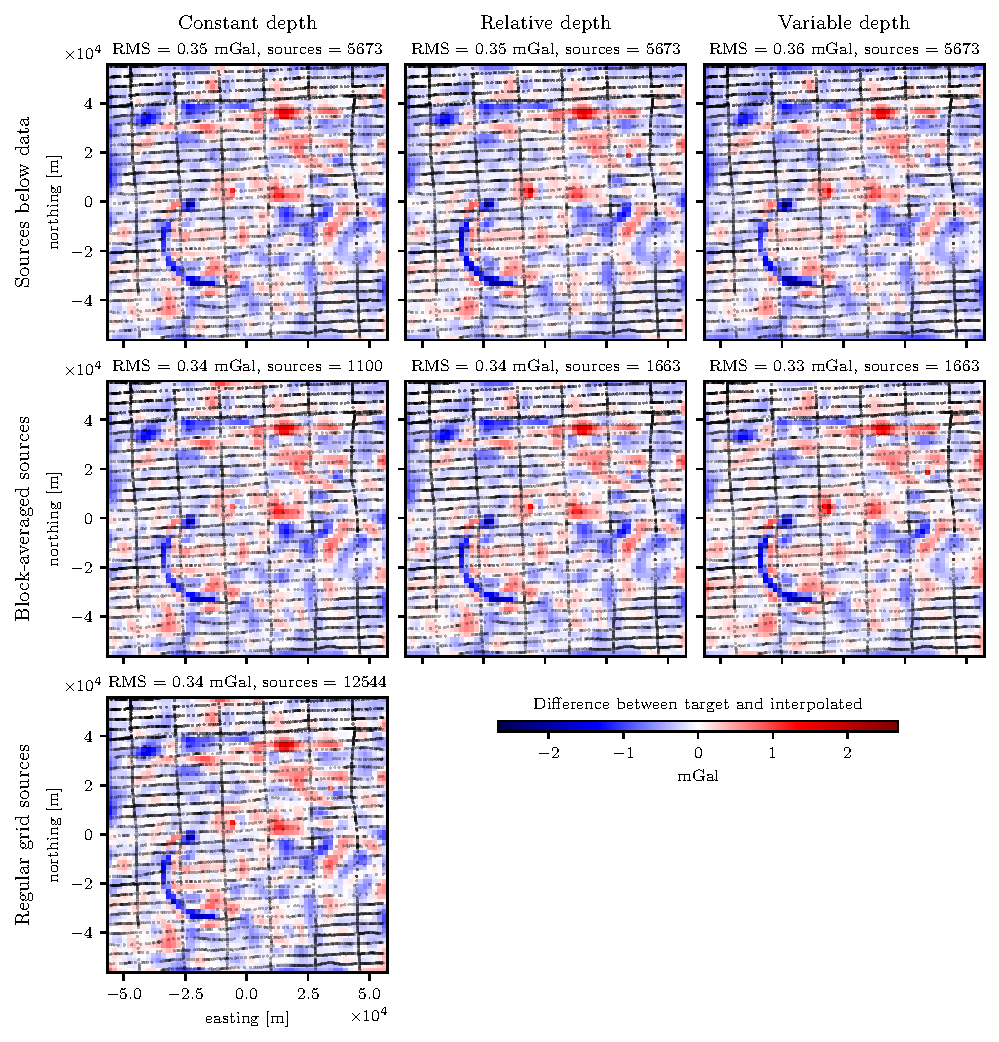
\includegraphics[width=\linewidth]{figs/airborne_survey_differences.pdf}
    \caption{
        Pseudo-color maps of the differences between the target grid and the
        interpolated synthetic airborne survey data produced by each source
        distribution strategy.
        The black dots represent the horizontal location of the synthetic data
        points. The RMS error and total number of equivalent sources is
        reported for each strategy at the top of the respective maps.
    }
    \label{fig:airborne-survey-differences}
\end{figure*}

We investigated the effect on interpolation accuracy of different strategies
for distributing the equivalent sources horizontally and vertically.
To do this, we used the damped least-squares solution described in
Section~\ref{sec:eql_inversion} (without gradient boosting) to interpolate the
synthetic datasets (Fig.~\ref{fig:synthetic-layouts}) and compared the results
against the target grid (Fig.~\ref{fig:synthetic-target}).
This process was repeated for each combination of horizontal layout
(\emph{sources below data} and \emph{block-averaged sources}) and depth type
(\emph{constant}, \emph{relative}, and \emph{variable}) and for regular grid
sources with a constant depth, totalling 7 different combinations.

Each source distribution strategy requires certain hyper-parameters to be
chosen in order to build the set of point sources.
For example, using a constant depth needs the definition of the depth and using
block-averaged sources requires the definition of the block size.
The predictive capabilities of the equivalent sources depend on the choice of
these hyper-parameters.
To ensure that our comparisons are fair, we perform an exhaustive search over
combinations of hyper-parameter values (including the damping parameter from
Eq.~\ref{eq:misfit}) to obtain the best prediction that can be achieved by each
source distribution strategy.
Here, the best prediction is defined as the one that minimizes the root
mean-square error (RMS) between interpolated values and the target grid
(Fig.~\ref{fig:synthetic-target}).
The parameter values used in these searches and the one producing the smallest
RMS error are outlined in Tables~\ref{tab:parameters-ground-survey}
and~\ref{tab:parameters-airborne-survey}.

Fig.~\ref{fig:ground-survey-differences}
and~\ref{fig:airborne-survey-differences} show the differences between the
target grid and the best prediction achieved by each source distribution
strategy for the ground and airborne synthetic surveys, respectively.
For the synthetic ground survey, the horizontal layouts produced similar RMS
values of approximately 0.8\mGal{} regardless of the depth type, with the
exception of the regular grid layout which produced a larger RMS of
\BestGroundGridSourcesConstantDepthRms{}\mGal{}.
The differences between the target grid and the interpolated values are larger
in regions of poor data coverage.
Edge effects are present for all strategies but are noticeably smaller for the
combination of block-averaged sources with a variable depth based on the
nearest neighbour distance.
For the synthetic airborne survey, all strategies (including the regular grid)
produced similar RMS errors of approximately 0.3\mGal{}.
The maps of the differences between the target grid and interpolation results
are visually indistinguishable from each other.

%%%%%%%%%%%%%%%%%%%%%%%%%%%%%%%%%%%%%%%%%%%%%%%%%%%%%%%%%%%%%%%%%%%%%%%%%%%%%%%


\subsection{Window size and overlap in gradient boosting}
\label{sec:window_size_and_overlap}

We assessed the trade-offs in interpolation accuracy and computation time of
the gradient-boosted equivalent sources algorithm as a function of the two key
controlling factors: the window size and the amount of overlap between adjacent
windows.
The comparisons were performed against a regular least-squares solution
(Eq.~\ref{eq:least_squares_solution}) using the synthetic airborne data
(Fig.~\ref{fig:synthetic-layouts}c-d).
To avoid biasing the results, we used the same locations of equivalent sources
for both the regular and gradient-boosted interpolations, namely
block-averaged sources with a block size of
\BestAirborneBlockAveragedSourcesRelativeDepthSpacing\m{} and a
relative depth of
\BestAirborneBlockAveragedSourcesRelativeDepthDepth\m{}.

\subsubsection{Window size}
\label{sec:window_size}

The size of the windows controls the size of the Jacobian matrices
$\tilde{\mathbf{A}}_k$ by limiting the number of data points and equivalent
sources used in each step of the gradient-boosting algorithm
(Alg.~\ref{alg:gradient_boosting_window}).
Thus, using smaller windows will reduce the total amount of computer memory
required to estimate the source coefficients.
Nevertheless, smaller windows may produce less accurate interpolations by
failing to achieve the global minimum of the goal function in
Eq.~\ref{eq:misfit}.
The window size might also impact the computation time in non-intuitive ways
since smaller windows generate smaller least-squares problems but also require
more gradient-boosting iterations.

We calculated the interpolation RMS error (between the interpolated grid and
the target grid in Fig.~\ref{fig:synthetic-target}) and computation time for a
fixed window overlap of 50\% and several window sizes.
To avoid any biases introduced by the shuffling of windows, the calculations
were repeated using different seeds for the pseudo-random number generator used
in the shuffling.
Fig.~\ref{fig:gradient-boosted-comparison}a shows the RMS error and
Fig.~\ref{fig:gradient-boosted-comparison}c shows the computation time
required for estimating the source coefficients, both as functions of
the window size.

\begin{figure*}[tb]
    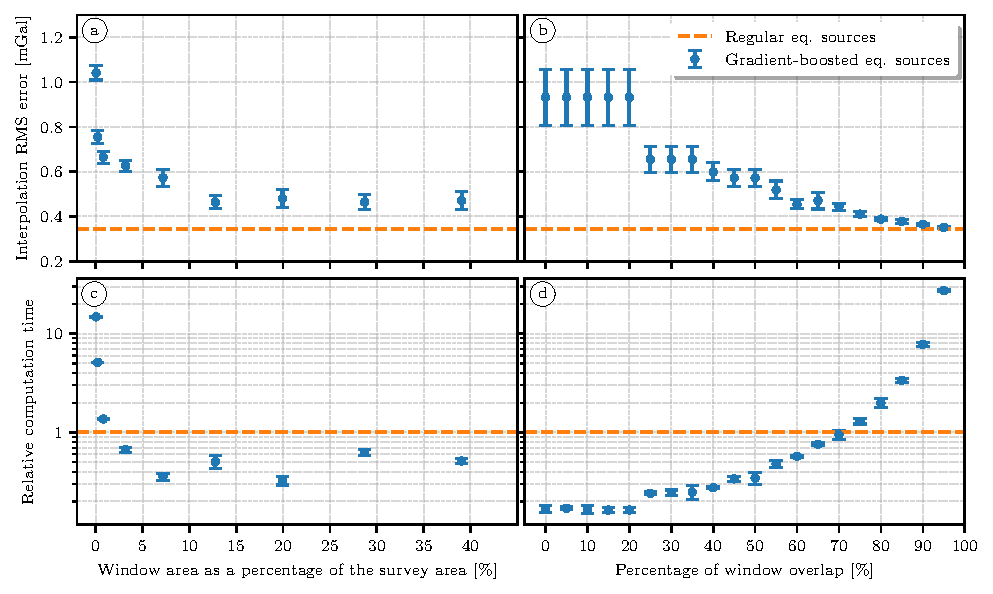
\includegraphics[width=\linewidth]{figs/gradient-boosted-comparisons.pdf}
    \caption{
        Interpolation RMS error (a-b) and relative computation time (c-d) for
        regular least-squares equivalent sources (orange dashed lines) and
        gradient-boosted equivalent sources (blue dots and error bars).
        Window overlap is given as a percentage of the window size (an overlap
        of 50\% means that two adjacent windows share an area half of the size
        of the entire window).
        For gradient-boosting, the RMS errors and computation times are the
        means (error bars are 1 standard deviation) of results using different
        seeds for the pseudo-random number generator.
        Computation time is the ratio between the time required to estimate the
        source coefficients for the gradient-boosted and the regular equivalent
        sources.
}
    \label{fig:gradient-boosted-comparison}
\end{figure*}

These results show that the interpolation error for gradient-boosting is
generally larger than the error for regular equivalent sources.
The error decreases asymptotically to within $\sim 40\%$ of the regular
equivalent sources for windows with an area greater than $\sim 10\%$ of the
survey area.
The computation time similarly decreases with window size, with the
gradient-boosting being generally faster than the regular equivalent sources
for windows with an area greater than $\sim 5\%$ of the survey area.
As the window size increases, both RMS error and computation time appear to
stabilize to nearly constant levels.

\subsubsection{Window overlap}

The amount of overlap between adjacent windows plays an important role in the
performance of the gradient-boosted equivalent sources.
It controls the number of iterations and how many times a particular source is
used in the least-squares fitting process.
The experiments in the previous section showed that 50\% overlap was
sufficient to achieve acceptable interpolation accuracy.
However, we studied separately the impacts of the amount of window overlap on
both accuracy and computation time.

We performed a similar experiment to the one in section~\ref{sec:window_size}
but this time kept the window size fixed to \BoostOverlappingWindowSize{} and
varied the amount of overlap from 0\% to 95\% with a step size of 5\%.
All other experimental procedures remained unchanged.
Fig.~\ref{fig:gradient-boosted-comparison}b shows the RMS error and
Fig.~\ref{fig:gradient-boosted-comparison}d shows the computation time
required for estimating the source coefficients, both as functions of
the window overlap.

Our results show that the interpolation RMS error decreases with the amount of
overlap, reaching the same accuracy as the regular equivalent sources at
approximately 90\% overlap.
On the other hand, the computation time increases with the amount of overlap,
becoming larger than that of the regular equivalent sources for overlaps
greater than 70\%.
This is expected since increasing the overlap adds iterations to the gradient
boosting algorithm without decreasing the individual least-squares problem
sizes to compensate.


\subsection{
    Interpolation with gradient boosting
}
\label{sec:gb_interpolation}

Finally, we applied the gradient-boosted equivalent sources to interpolate the
synthetic airborne survey (Fig.~\ref{fig:synthetic-layouts}).
As previously, we used the block-averaged sources layout with a block size of
\EqlBoostAirborneSpacing{}.
Based on the results from section \ref{sec:window_size_and_overlap}, we adopted
a window overlap of 50\% and a window size of \EqlBoostAirborneWindowSize{}.

We estimated the relative depth of the sources and the damping parameter by
comparing the predictions against the values of the target grid.
The search explored \emph{depth} values between \EqlBoostAirborneMinDepth{} and
\EqlBoostAirborneMaxDepth{} and \emph{damping} values between
\EqlBoostAirborneMinDamping{} and \EqlBoostAirborneMaxDamping{} by steps of one
order of magnitude.
The most accurate predictions achieved a RMS error of
\EqlBoostAirborneRmsScore{} with a depth of \EqlBoostAirborneDepth{} and
a damping of \EqlBoostAirborneDamping{}.
It is worth noting that the RMS error achieved by the gradient-boosted
equivalent sources is comparable to the ones obtained by the regular equivalent
sources in Section \ref{sec:synthetic_distributions}.
To highlight the importance of randomizing the order of windows in the
gradient-boosting iterations, we preformed the interpolation once more using
the same values of \emph{damping} and \emph{depth} but this time iterating over
windows in sequential order (South to North, West to East).

\begin{figure}[tb]
    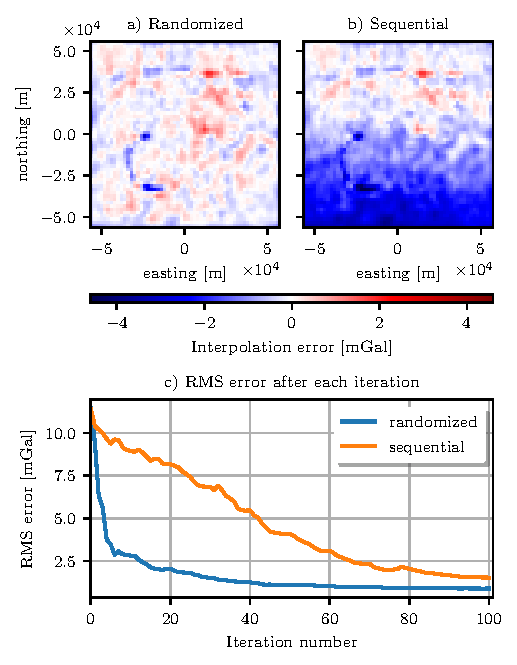
\includegraphics[width=\linewidth]{figs/eql-boost-airborne.pdf}
    \caption{
        Interpolation error for gradient-boosted equivalent sources using
        randomized (a) and sequential (b) window order.
        (a and b)~Pseudo-color maps of the differences between the target grid
        and the interpolated synthetic airborne survey data.
        The color scale has been cropped to the same range as
        Fig.~\ref{fig:airborne-survey-differences}.
        (c)~Root-mean squared error after each iteration of the
        gradient-boosting algorithm.
}
\label{fig:eql-boost-airborne}
\end{figure}

Figs.~\ref{fig:eql-boost-airborne}a-b show the differences between the target
grid and the interpolation results for windows in randomized and sequential
order, respectively.
The differences for randomized windows resemble those for regular least-squares
equivalent sources seen in Figs.~\ref{fig:ground-survey-differences} and
\ref{fig:airborne-survey-differences}.
On the other hand, the differences for sequential windows show a clear
trend of large negative differences in the South decreasing towards the North.
This trend is correlated with the order in which windows are executed, with
differences decreasing in absolute value towards the end of the algorithm.
Fig.~\ref{fig:eql-boost-airborne}c shows the RMS error of the fitting process
after each iteration for both window orders, clearly indicating that
a randomized window order leads to faster convergence of the algorithm.


%%%%%%%%%%%%%%%%%%%%%%%%%%%%%%%%%%%%%%%%%%%%%%%%%%%%%%%%%%%%%%%%%%%%%%%%%%%%%%%

\section{Gridding gravity data from Australia}

\begin{figure*}[p]
    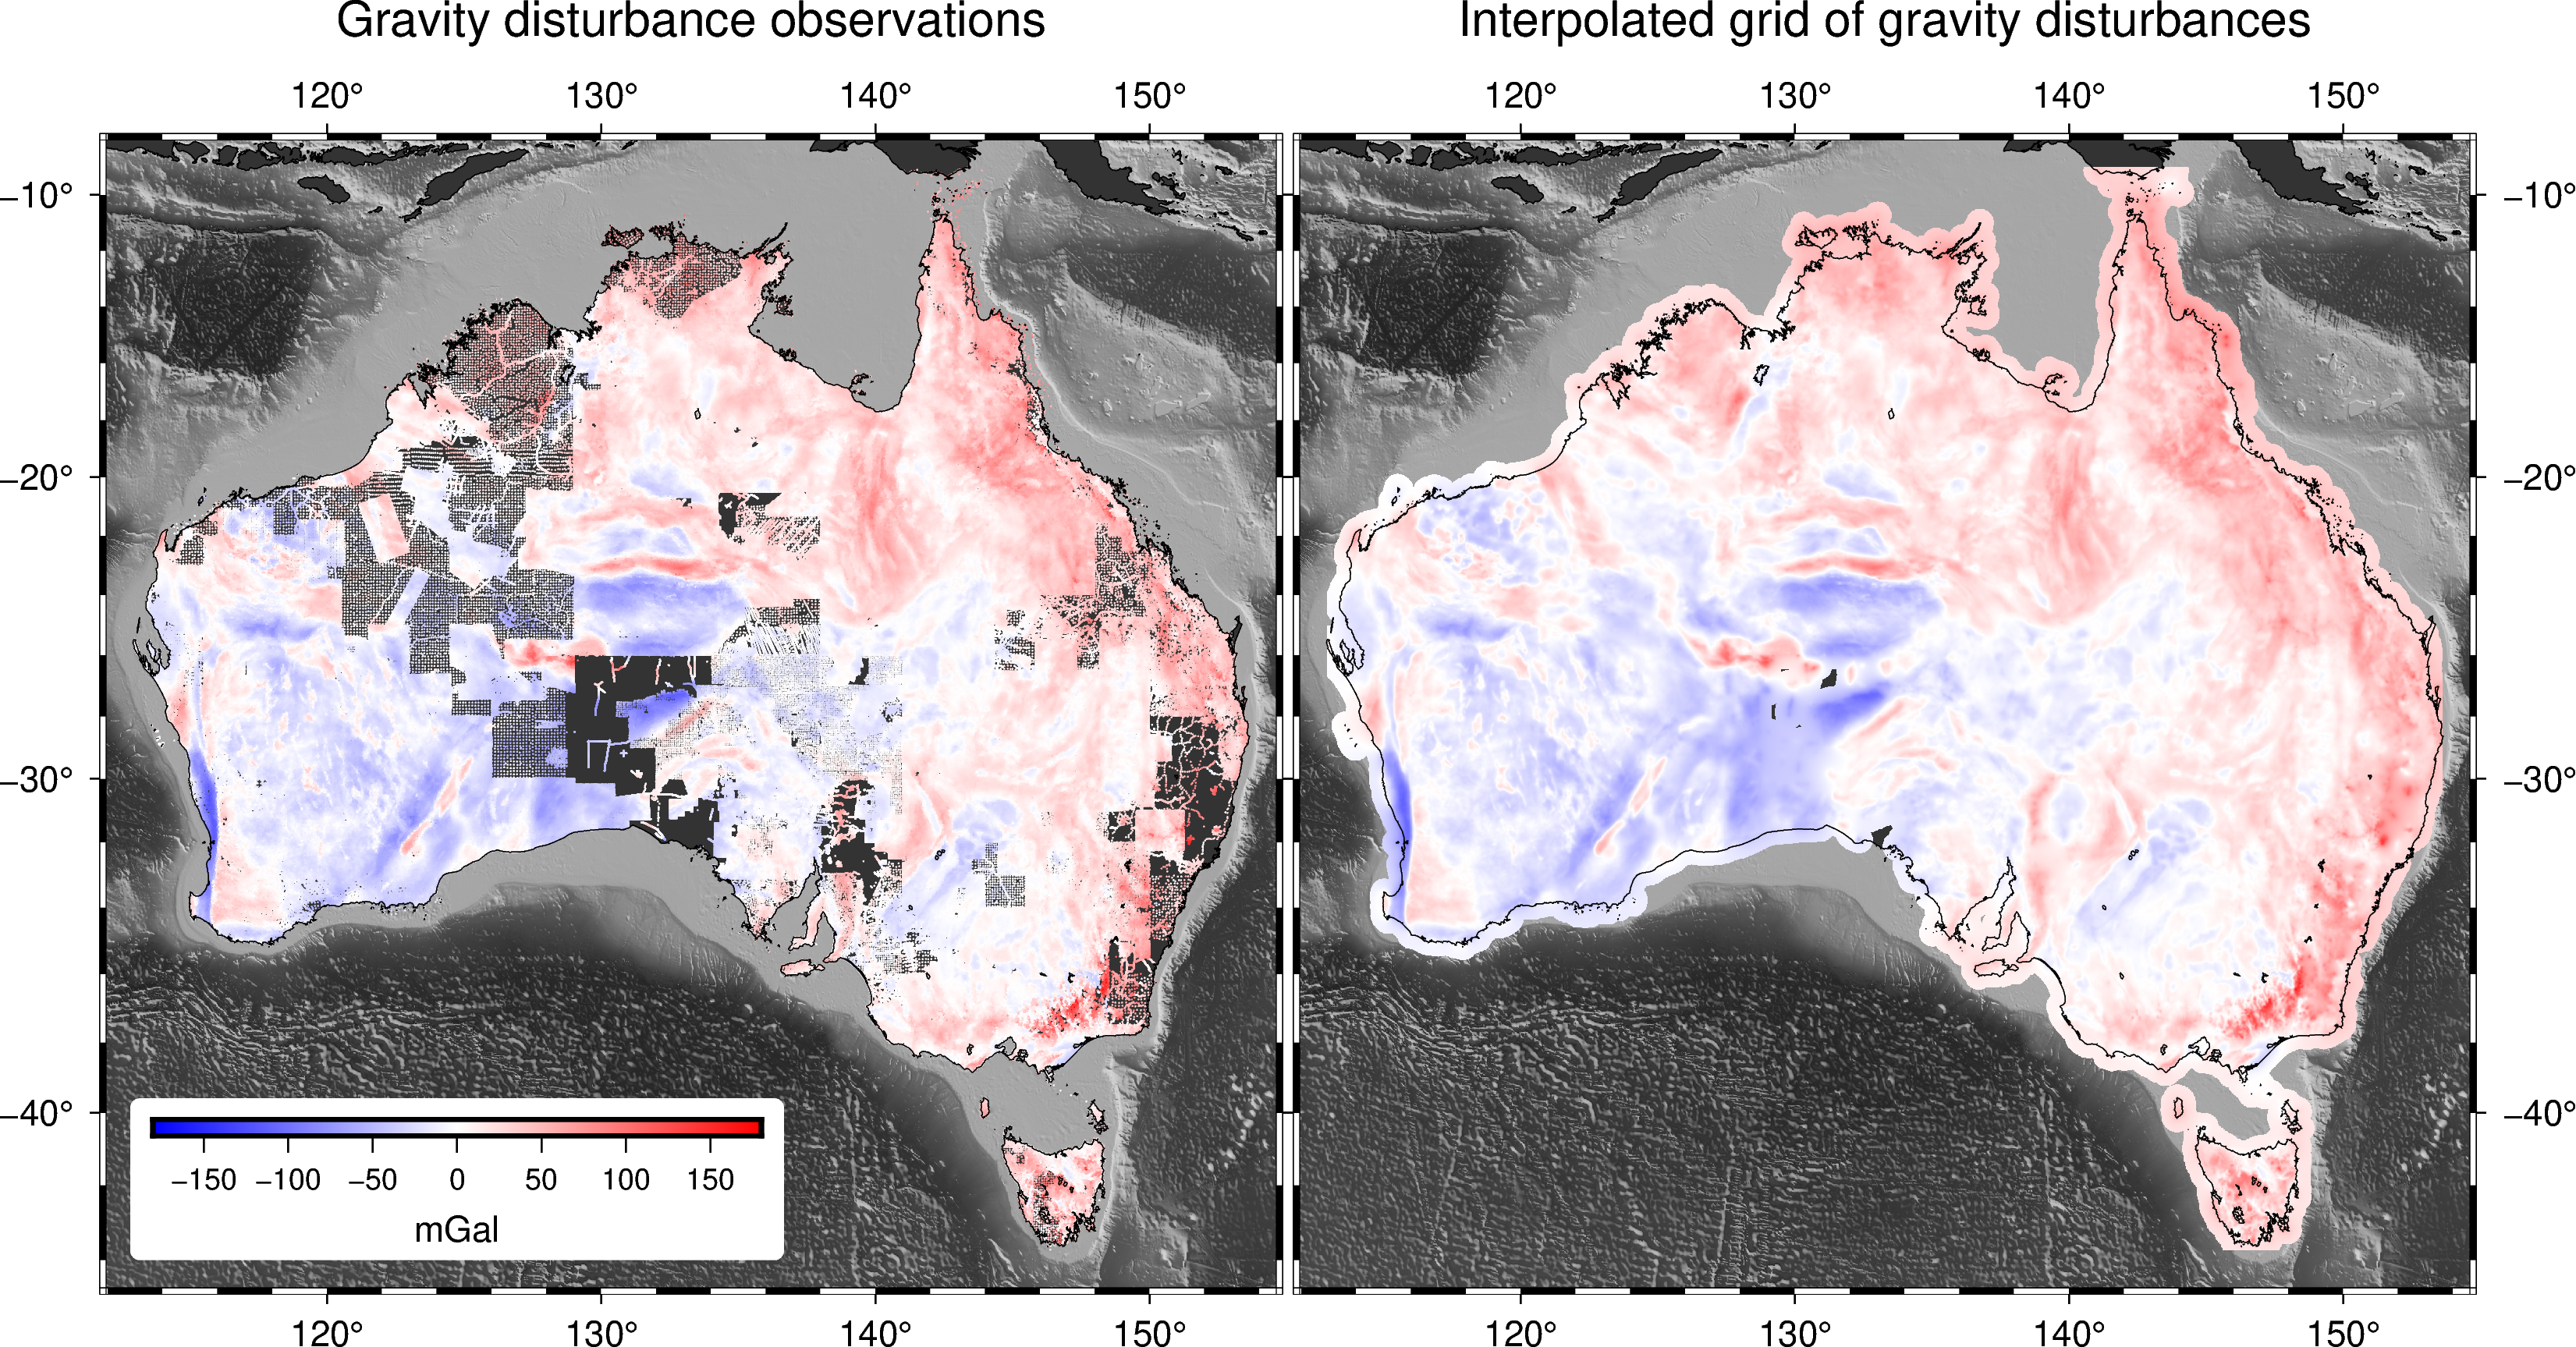
\includegraphics[width=\linewidth]{figs/australia.png}
    \caption{
      Pseudo-color maps of observed (a and c) and
      interpolated (b and d) gravity disturbance of Australia.
      The observed values in a and c are plotted as colored circles.
      The red rectangle marks the boundaries of the highlight maps in c
      and d.
      Observations are part of a compilation by \citet{wynne2018} of
      over 1.7 million ground gravity measurements.
      Interpolated values were obtained through gradient-boosted equivalent
      sources and calculated on a regular grid at \AustraliaEqlGridHeight{}
      over the WGS84 ellipsoid.
    }
    \label{fig:australia}
\end{figure*}

This section will demonstrate how gradient-boosted equivalent sources can be
used to interpolate large datasets onto regular grids at uniform height.
For this purpose, we selected an open-access compilation of ground gravity
surveys over Australia made by \citet{wynne2018} and filtered and referenced to
the WGS84 ellipsoid by \citet{australia_compilation}.
It contains over 1.7 million data points and covers most of the Australian
territory at variable point spacings.
Our goal is to create a 1~arc-minute resolution grid of gravity disturbances at
a constant geometric height of \AustraliaEqlGridHeight{} (the largest height of
observations).

We computed the gravity disturbance by removing the normal gravity of
the WGS84 ellipsoid from the observed gravity data (Fig.~\ref{fig:australia}).
Here, normal gravity was computed at each observation point through the
closed-form formula of \citet{ligotze2001} using the Boule software
\citep{boule2020}.
Finally, we converted the observations to planar Cartesian coordinates by
applying a Mercator projection.

We start the interpolation process by defining a set of block-averaged sources
using a block size of 1.8\km{}, resulting in a total of
\AustraliaEqlNSources{}~point sources.
The block size was chosen to match the desired resolution of the final grid
(1~arc-minute is approximately 1.8\km{} at the equator).
Based on the results obtained in Section~\ref{sec:synthetic_distributions}, we
have chosen to use the \emph{relative depth} strategy.
The window overlap was once again fixed at 50\%.
To determine the size of the windows, we calculated the amount of computer memory
needed to store the largest Jacobian matrix for different values of window size
(Fig.~\ref{fig:australia-memory-cv-error}a).
We have chosen a size of \AustraliaEqlWindowSize{} in order to limit the
amount of memory needed to under 16~Gigabytes.

\begin{figure}[tbh!]
    \makeatletter%
    \if@twocolumn%
        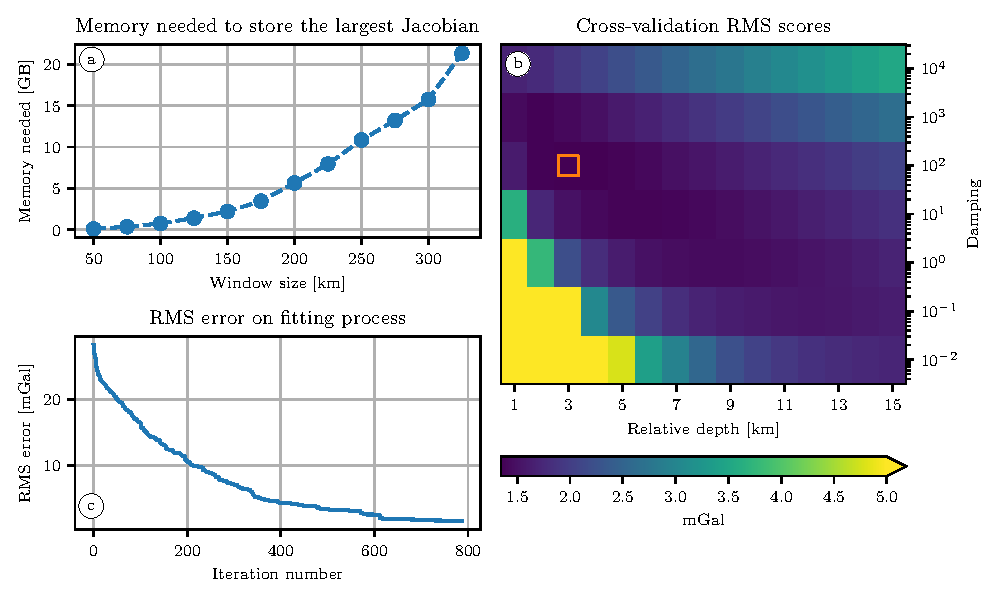
\includegraphics[width=\linewidth]{figs/australia-memory-cv-error.pdf}
    \else% \@twocolumnfalse
        \centering
        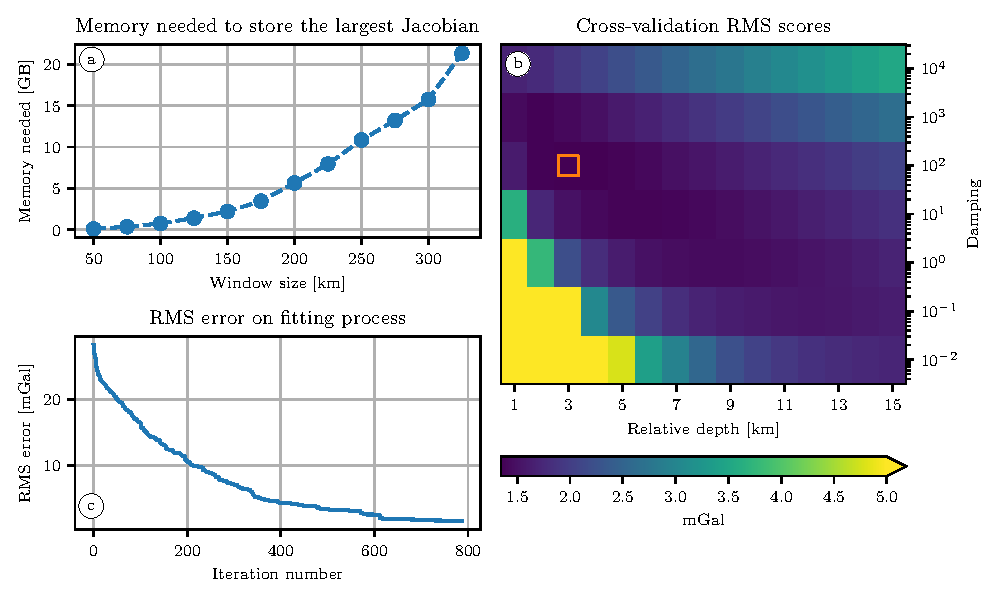
\includegraphics[width=0.6\linewidth]{figs/australia-memory-cv-error.pdf}
    \fi
    \makeatother
    \caption{
        (a) Amount of computer memory needed to store the largest Jacobian
        matrix for different window sizes. Our implementation uses double
        precision floating point numbers (64 bits) for the Jacobian.
        (b) Root-mean square error against the observed data after each
        iteration of the gradient-boosting algorithm.
        (c) K-Fold cross-validation root-mean square errors obtained for each
        pair of damping and depth parameters. The orange star highlights the
        minimum.
    }
    \label{fig:australia-memory-cv-error}
\end{figure}

We determined the depth of the sources and the damping parameter by applying
K-Fold cross-validation through the scikit-learn library \citep{sklearn2011}.
The method randomly divides the original data into $k$ sets (folds), fits the
model using only data from $k - 1$ folds, and validates the model by comparing
its predictions against the one remaining fold.
This process is carried out once for each one of the $k$ folds, leading to
an estimated mean cross-validation RMS error for the model.
To speed up the computation, we only performed the cross-validation on a subset
of the data corresponding to an area of
\AustraliaSmallAreaEastingSize{}$\times$\AustraliaSmallAreaNorthingSize{}
containing \AustraliaSmallAreaNPoints{} points.
We ran the cross-validation repeatedly for combinations of \emph{depth},
ranging from \AustraliaDepthMin{} to \AustraliaDepthMax{},
and \emph{damping}, from \AustraliaDampingMin{} to \AustraliaDampingMax{} in
steps of one order of magnitude.
Figure \ref{fig:australia-memory-cv-error}c shows the resulting
cross-validation RMS errors and highlights the minimum value of
\AustraliaEqlRmsScore{}, which corresponds to a relative depth of
\AustraliaEqlDepth{} and a damping equal to \AustraliaEqlDamping{}.

Finally, we proceeded to estimate the source coefficients using the entire
dataset and the parameters previously determined.
The estimated source coefficients were then used to predict the values of the
gravity disturbance on a regular grid of
\AustraliaEqlGridNLongitude{}$\times$\AustraliaEqlGridNLatitude{} points at
\AustraliaEqlGridHeight{} above the ellipsoid.
On a modest workstation with 16 cores and 16~Gigabytes of RAM,
estimating the \AustraliaEqlNSources{} coefficients with gradient-boosting took
$\sim 1.3$~hours and the prediction step took $\sim 18$~minutes.

Fig.~\ref{fig:australia} shows the original data distribution and the
interpolated grid.
Grid points that are further than 50\km{} from the nearest data point are
masked to avoid unrealistic extrapolations.
Fig.~\ref{fig:australia-memory-cv-error}b shows the RMS error against the
observed data after each iteration of the algorithm.
Fig.~\ref{fig:australia-residuals} shows the difference between the observed
and predicted gravity disturbances.
The inset figure shows a histogram of these residuals, which are approximately
normally distributed around zero.

\begin{figure}[tb]
    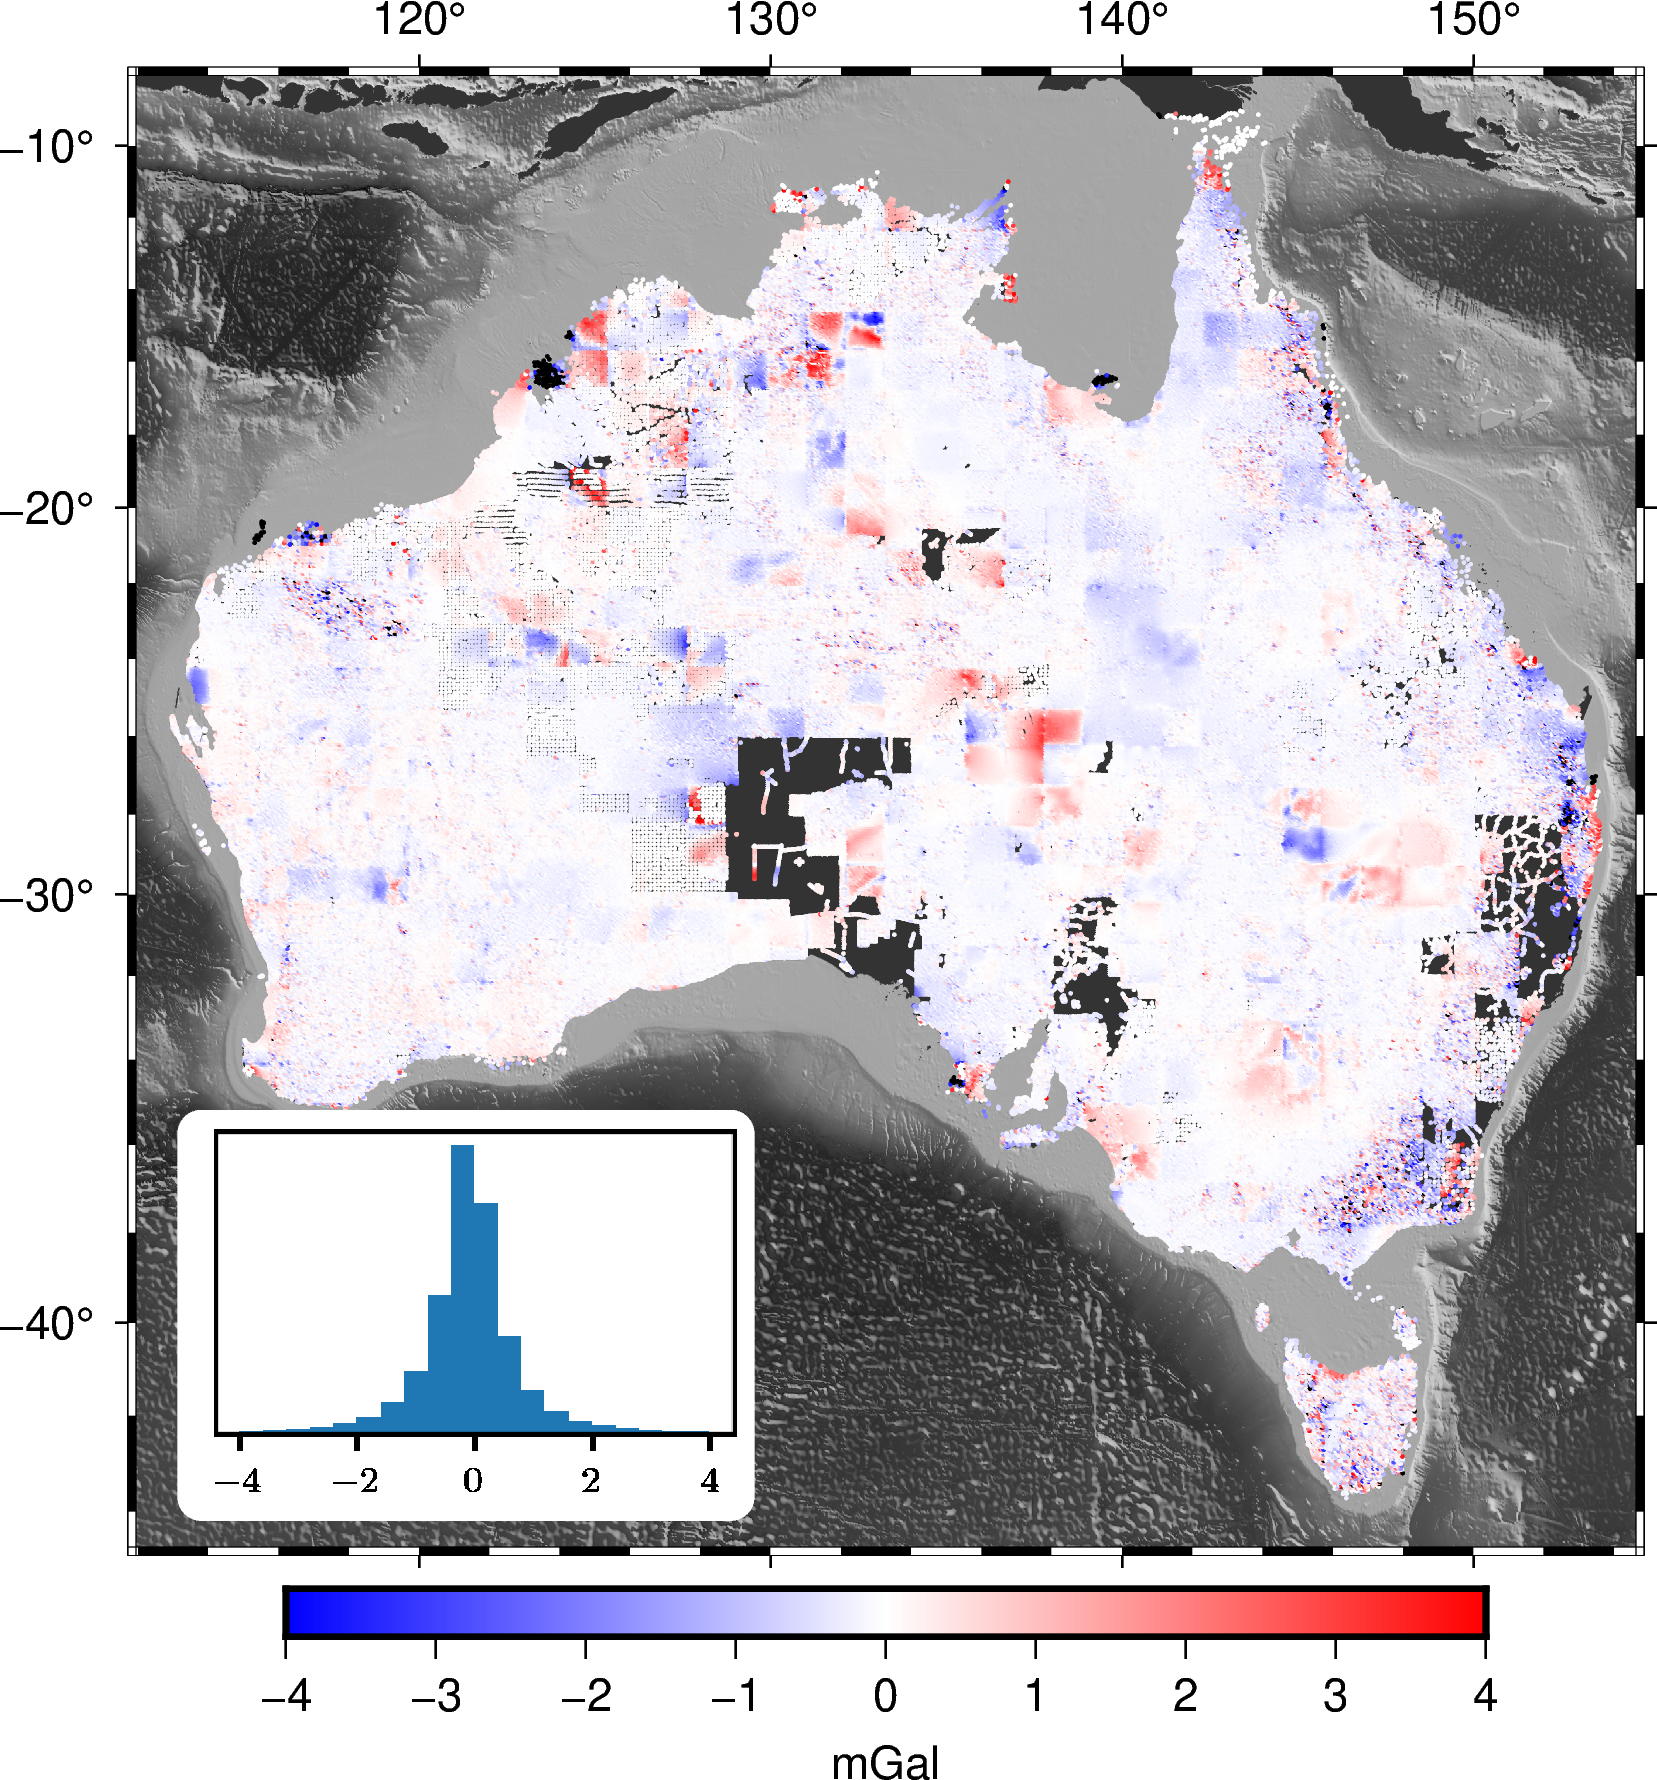
\includegraphics[width=\linewidth]{figs/australia-residuals.png}
    \caption{
        Residuals. Differences between the gravity disturbance data from
        Australia and the predicted values by the estimated equivalent sources
        on the same observation points. The color map has been truncated to
        improve the visualization around the largest portion of residual
        values. The inset plot shows a histogram of the residuals.
    }
    \label{fig:australia-residuals}
\end{figure}


%%%%%%%%%%%%%%%%%%%%%%%%%%%%%%%%%%%%%%%%%%%%%%%%%%%%%%%%%%%%%%%%%%%%%%%%%%%%%%%

\section{Discussion}

\subsection{Location of sources}

The results of our tests on synthetic data
(Figs.~\ref{fig:ground-survey-differences}
and~\ref{fig:airborne-survey-differences}) show that there are no significant
differences in interpolation accuracy between source distribution strategies,
both in terms of the interpolation RMS errors and from visual inspection of the
difference maps.
Therefore, we conclude that all source distribution strategies are able to
produce comparable interpolations.
Nevertheless, the \emph{block-averaged sources} strategy makes use of fewer
sources when compared with other strategies, which reduces the computational
load of estimating the sources coefficients and forward modelling.
To ensure that the interpolation is able to reproduce the high frequencies in
the data, the block size used in the averaging should be chosen to match the
desired grid resolution.

The choice of source depth strategy does not appear to significantly impact the
interpolation RMS error.
In the particular case of a sparse ground survey with block-averaged sources,
the use of a variable depth visibly reduced edge effects and artifacts in areas
of poor data coverage.
At a first glance, the choice of a depth strategy would not seem to impact
the computation time.
However, when searching for the set of hyper-parameters that produce the most
accurate interpolation (e.g., through cross-validation), one must solve the
inverse problem once for every possible combination of parameters.
A depth strategy like the \emph{variable depth} requires a higher number of
hyper-parameters (depth shift $\Delta z$, depth factor $\alpha$, and the number
of nearest neighbours $k$ from Eq.~\ref{eq:variable_depth}) than other
strategies which only require a single parameter.
Having more parameters means increasing the dimensions of the parameter space
and thus increasing the number of possible combinations.
Thus, we recommend using a \emph{constant depth} or a \emph{relative depth}
when processing large datasets in order to minimize computation time.

\subsection{Gradient boosting}

From Fig.~\ref{fig:gradient-boosted-comparison}a
and~\ref{fig:gradient-boosted-comparison}c, we can see that the
gradient-boosted equivalent sources produce slightly less accurate
interpolation results but are able to achieve smaller computation times than
regular equivalent sources.
The reduction of the accuracy might be due to the gradient boosting algorithm
failing to converge to the global minimum of the goal function.
As the windows increase in size, interpolation error decreases because more data
points are included into the least-squares fitting of the source coefficients.
At the same time, the fitting process becomes faster because of a reduction in
the number of iterations.
Our results indicate that it is desirable to maximize the window size,
which can be done up to the point that the Jacobian matrices still fit within
the available computer memory.

The results shown in Figs.~\ref{fig:gradient-boosted-comparison}b
and~\ref{fig:gradient-boosted-comparison}d indicate that using
window overlap values between 40\% and 70\% strike a balance between
accuracy and computation time.
This corroborates our initial choice of 50\% overlap, which is good enough for
producing accurate predictions in reasonable times.

Finally, the results in Fig.~\ref{fig:eql-boost-airborne} highlight the
importance of randomizing the order in which the overlapping windows are
iterated.
Running the gradient boosting algorithm sequentially produces less accurate
predictions and decreases the convergence rate of the method.

\subsection{Australia gravity data}

The application of the gradient-boosted equivalent sources to the Australian
gravity dataset demonstrates that the method is able to interpolate and
upward-continue large datasets in a reasonable amount of time using only modest
computational resources.
The resulting grid (Fig.~\ref{fig:australia}) preserves the high resolution of
the original data while avoiding aliasing artifacts due to the block averaging
of the source locations.
Some parts of the grid are smoother and have lower amplitudes than the original
data (e.g., some southwestern parts), which is expected from the upward
continuation that was performed to have the grid at a constant height.
From the cross-validation analysis on a subset of the data, we estimate that
the interpolation error is approximately \AustraliaEqlRmsScore{}.

The largest residuals in Fig.~\ref{fig:australia-residuals} are located in
regions with high-amplitude short-wavelength features in the observed data.
This is expected since the method involves some degree of smoothing because of
the use of damping and the source depths.
There are also low-amplitude long-wavelength residual signals that seem to
coincide with some of the windows of the gradient-boosting method.
A possible cause of these features is inability of the equivalent-sources
within a window to adequately fit the long-wavelength components of the data.
We note, however, that all of these long-wavelength residuals are smaller than
1\mGal{} in amplitude and do not represent a significant source of errors.

The elongated valley around the minimum of the cross-validation RMS errors
(Fig.~\ref{fig:australia-memory-cv-error}c) shows that there is ambiguity in
the choice of damping and source depths.
One could choose a large damping with a small depth or a small damping with a
large depth to achieve roughly the same interpolation result.
This is expected since both parameters control the smoothness of the
interpolation.

%%%%%%%%%%%%%%%%%%%%%%%%%%%%%%%%%%%%%%%%%%%%%%%%%%%%%%%%%%%%%%%%%%%%%%%%%%%%%%%

\section{Conclusions}

The equivalent source technique has been proven to be well suited for
interpolating gravity disturbances and magnetic anomalies.
The two main reasons that make it to stand out from other 2D interpolation
methods is the fact that the equivalent sources take into account the height of
the observations and that the interpolated values will always be harmonic
functions.
The main challenge of using equivalent sources in practice is the high
computational load of estimating the coefficients of the equivalent sources,
specially the computer memory needed to store the Jacobian matrix.

We present two strategies that could be simultaneously applied to interpolate
datasets with millions of points on modest hardware:
block-averaging source locations, which reduces the number of equivalent
sources needed for the interpolation,
and the gradient-boosted equivalent source algorithm, which breaks down the
inverse problem into smaller sets of equivalent sources defined by overlapping
windows.
Both methods were tested against synthetic datasets in order to compare their
accuracy and how they perform in terms of computational efficiency.

Our results show that the block-averaged sources reduce the computational
load needed to estimate source coefficients in comparison to two traditional
strategies (placing sources below data points or on regular grids).
We also show that this reduction of the number of sources does not affect
the accuracy of the predictions.
The use of block-averaged sources may also prevent aliasing of the interpolated
values, specially when the observations are unevenly sampled (e.g., airborne
and shipborne surveys).
Special attention must be payed when choosing the size of the blocks for
averaging.
As a thumb rule, we recommend choosing a size approximately equal to
the resolution of the regular grid where the values will be interpolated.

Tests that compared strategies for the vertical location of the
sources showed that any one of the three strategies tested
(\emph{constant depth}, \emph{relative depth} and \emph{variable depth})
produces comparable accuracy of interpolation.
Nevertheless, we are more prone to recommending either the \emph{constant
depth} or the \emph{relative depth} for most applications because they involve
less hyper-parameters that would need to be configured before the actual
interpolation.

Gradient-boosted equivalent sources were shown to heavily reduce the computer
memory needed to estimate source coefficients, making it possible to
interpolate large datasets with millions of points that would otherwise produce
Jacobian matrices larger than the available memory.
The interpolations obtained though this new method achieve close to the same
accuracy than the regular equivalent sources, while reducing the computation
time by approximately a factor of three.
We also show that an overlap of 50\% between adjacent windows achieves a good
compromise between accuracy and computation time.
The size of the overlapping windows should be chosen as the maximum value
possible that creates Jacobian matrices that still fit into computer memory.
Moreover, randomizing the order in which the windows are iterated increases the
convergence rate of the algorithm and is essential to producing accurate
predictions.

The gradient-boosting method can be used in conjunction with any horizontal
source layout, depth strategy, or source type (e.g., point sources, prisms,
tesseroids) because it does not rely on assumptions about the sources.
Future research should investigate the application of gradient boosting to
other equivalent source methods.

%%%%%%%%%%%%%%%%%%%%%%%%%%%%%%%%%%%%%%%%%%%%%%%%%%%%%%%%%%%%%%%%%%%%%%%%%%%%%%%

\section{Data and code availability}

The Python source code used to produce all results and figures presented here
is available at
\url{https://doi.org/10.6084/m9.figshare.13604360} and
\url{https://github.com/compgeolab/eql-gradient-boosted}
under the BSD 3-clause open-source license.

The gradient-boosted equivalent sources implementation is based on the
equivalent source code in the Harmonica library \citep{harmonica2020}.
Other software used in this study includes:
Pooch \citep{pooch2020} for downloading and caching datasets,
Verde \citep{verde2018} for block reductions and coordinate manipulations,
Boule \citep{boule2020} for normal gravity calculations,
xarray \citep{xarray2017} and Numpy \citep{numpy2020} for handling
multidimensional arrays and numerical computations,
Numba \citep{numba2015} for just-in-time compilation and parallelization,
scikit-learn \citep{sklearn2011} for cross-validation,
Matplotlib \citep{matplotlib2007} and PyGMT \citep{pygmt2020} for generating
the figures and maps,
and the Jupyter notebook programming environment \citep{jupyter2016}.
Harmonica, Boule, Pooch, and Verde are part of the Fatiando a Terra project
\citep{fatiando2013}.

All datasets used are open-access and publicly available.
The synthetic surveys were generated using
a public domain gravity dataset for Southern Africa distributed by the
NOAA NCEI (\url{https://www.ngdc.noaa.gov/mgg/gravity/gravity.html})
and the Great Britain Aeromagnetic
Survey distributed by the
British Geological Survey (BGS) under an Open Government License
(\url{https://www.bgs.ac.uk/products/geophysics/aeromagneticRegional.html}).
The shaded relief in Fig.~\ref{fig:australia} is the SRTM15+ dataset by
\citet{tozer2019}.
The Australian ground gravity
data is based on a compilation distributed by Geoscience Australia under a
Creative Commons Attribution 4.0 International Licence \citep{wynne2018}  which
was filtered and referenced to the WGS84 ellipsoid by
\citet{australia_compilation} and is distributed under the same license
(\url{https://doi.org/10.6084/m9.figshare.13643837}).


%%%%%%%%%%%%%%%%%%%%%%%%%%%%%%%%%%%%%%%%%%%%%%%%%%%%%%%%%%%%%%%%%%%%%%%%%%%%%%%

\section{Acknowledgements}

We are indebted to the developers and maintainers of the open-source software
without which this work would not have been possible.
We would also like to thank Editor Frederik Simons, Assistant Editor Fern
Storey, and two anonymous reviewers for their constructive comments.
S.R. Soler is supported by a scholarship from CONICET, Argentina.
This work contains British Geological Survey materials ©~UKRI.
S.R. Soler and L. Uieda jointly developed the initial idea, analysed the
results, and wrote the paper. S.R. Soler produced all results and developed the
software implementation with the assistance of L. Uieda.
